\documentclass[11pt,twoside]{article}

\usepackage[margin=1in]{geometry}
\usepackage{amsmath,amssymb,amsthm,mathtools}
\usepackage[inline,shortlabels]{enumitem}
\usepackage{xcolor}
\usepackage{../misc_files/course-definition-boxes}
\usepackage{microtype}

% Revision date: maintained by scripts/build_lecture_notes.py. Keep this command.
\newcommand{\lecturerevised}{2026-11-24 22:19 UTC-06:00}
\usepackage{eso-pic}
\AddToShipoutPictureBG{%
  \AtPageLowerLeft{%
    \put(\LenToUnit{0.5\paperwidth},\LenToUnit{0.5in}){%
      \makebox(0,0){\normalfont\footnotesize\color{black!60}Last revised: \lecturerevised}%
    }%
  }%
}

\usepackage[square,authoryear]{natbib}
\usepackage[colorlinks=true,linkcolor=blue!60!black,
  urlcolor=blue!60!black,citecolor=blue!60!black]{hyperref}
\usepackage[nameinlink,capitalize]{cleveref}
\crefname{exercise}{Exercise}{Exercises}
\Crefname{exercise}{Exercise}{Exercises}

\usepackage{../exercises/course-exercises}
\usepackage{array,booktabs,needspace}
\usepackage{tikz}
\usetikzlibrary{arrows.meta}

% Short refinements that may be skipped on a first reading.
\usepackage{enotez}
\DeclareInstance{enotez-list}{lecture}{list}{format=\normalsize,number={#1.}}
\setenotez{list-name=Endnotes,list-style=lecture,backref=true}
\crefname{endnote}{Endnote}{Endnotes}
\Crefname{endnote}{Endnote}{Endnotes}


\definecolor{courseblue}{HTML}{17365D}
\newcommand{\E}{\mathbb E}
\newcommand{\I}{\mathbb I}
\renewcommand{\P}{\mathbb P}
\newcommand{\R}{\mathbb R}
\newcommand{\KL}{D}
\newcommand{\TV}{\mathrm{TV}}
\makeatletter
\@for\@letter:=A,B,C,D,E,F,G,H,I,J,K,L,M,N,O,P,Q,R,S,T,U,V,W,X,Y,Z\do{%
  \expandafter\edef\csname c\@letter\endcsname{\noexpand\mathcal{\@letter}}}
\makeatother
\newcommand{\lecturenumber}{19}

\newtheorem{theorem}{Theorem}[section]
\newtheorem{proposition}[theorem]{Proposition}
\newtheorem{corollary}[theorem]{Corollary}
\theoremstyle{definition}
\newtheorem{definition}[theorem]{Definition}
\newtheorem{example}[theorem]{Example}
\theoremstyle{remark}
\newtheorem{remark}[theorem]{Remark}

\renewcommand{\thepage}{\lecturenumber--\arabic{page}}
\renewcommand{\thesection}{\lecturenumber.\arabic{section}}
\renewcommand{\theequation}{\lecturenumber.\arabic{equation}}

\pagestyle{myheadings}
\markboth{Lecture \lecturenumber: Preference models and objectives}
{Lecture \lecturenumber: Preference models and objectives}

% Course-wide notation convention:
% Every vector is a column vector. If a matrix stores one vector per position,
% row i contains the transpose of that vector. Write every row-shaped vector
% explicitly as the transpose of a column vector.
% Use n for the number of independent training examples. Use sentence case in
% optional theorem titles. Use example environments for worked examples that
% are referenced later. Reserve \boxed{} for literal boxes in diagrams.

\hypersetup{pdftitle={Lecture 19: Preference models and objectives},
  pdfauthor={Csaba Szepesvari}}
\begin{document}
\raggedbottom

\begin{center}
\fcolorbox{courseblue}{white}{%
\begin{minipage}{0.92\textwidth}
\vspace{1mm}
\textbf{CMPUT 654: Mathematical Foundations of Modern AI Systems}
\hfill Fall 2026

\vspace{3mm}
\begin{center}
{\Large\bfseries Lecture \lecturenumber: Preference models and objectives}

\vspace{1mm}
November 5, 2026
\end{center}

\vspace{2mm}
\textit{Lecturer: Csaba Szepesv\'ari}
\hfill
\textit{Notes prepared by: Csaba Szepesv\'ari}
\vspace{1mm}
\end{minipage}}
\end{center}

What do pairwise preferences identify, and what are preference objectives
optimizing? Demonstrations supply behavior to imitate; comparisons assess
candidate responses. Under a scalar logistic model, connected comparisons
identify reward differences. A reference policy and a KL penalty determine
an optimal response distribution, which motivates direct preference
optimization (DPO). The lecture also shows how model misspecification,
restricted policy classes, and missing comparisons limit these conclusions.

\noindent\textbf{Reading guide.}
We first study the comparison experiment and identification, then population
fitting, the regularized optimum, and DPO. The prerequisites are binary log
loss and KL divergence from \href{lecture03.pdf}{Lecture 3}, misspecification
from \href{lecture07.pdf}{Lecture 7}, and demonstration and policy terminology
from \href{lecture18.pdf}{Lecture 18}. We work at one fixed prompt with
finitely many responses; generalization across prompts is outside the
results. Linked exercises develop the calculations behind the examples
and counterexamples. The appendices on broader preference models and the graph-cycle
condition may be skipped on a first reading.

\section{From demonstrations to comparisons}
\label{sec:comparisons}

Behavior cloning fits the responses a teacher produces. Preference learning
instead fits judgments about candidate responses. Separating the response
distribution from the judgment distribution is necessary to identify the
statistical target before choosing an optimization objective.

\emph{Fine-tuning} continues parameter training from an existing checkpoint.
\emph{Post-training} is the stage after pretraining and can contain several
fine-tuning procedures. In \emph{supervised fine-tuning} (SFT), the model fits
example responses by log loss, as in Lecture 18's behavior cloning.
Preference fine-tuning instead uses judgments comparing candidate responses.
Online reward-based reinforcement learning generates responses and updates
the model using their scores; those scores can come from learned preferences
or from checks such as tests of generated code.

A preference judgment asks which of two responses to the same prompt an
evaluator would choose. Such judgments can help specify desired behavior
when writing a good response is harder than comparing two responses already
available. Preference methods are used in major language-model training
pipelines: Llama 3 uses repeated rounds of SFT and DPO, while Olmo 3-Think
uses SFT, DPO, and then reinforcement learning with verifiable rewards.
The examples establish practical use and show that preference fitting can
coexist with other training stages. The
\hyperref[sec:bibliographical-notes]{bibliographical notes} give the sources
and describe modifications to the basic DPO objective.

Fix a prompt $u$ and a finite set $\cY$ of possible complete responses,
with $|\cY|\ge2$. We suppress $u$ in notation until discussing language-model
updates. A \emph{policy} is a probability mass function
$\pi\in\Delta_{\cY}$ on the complete responses. Treating a response as one
action retains the distribution generated by its successive token choices;
the present analysis concerns how the complete response is evaluated.

We receive preference feedback about pairs of possible responses. Model one
observation by jointly distributed random variables $(Y,Y',C)$ taking values
in $\cY^2\times\{0,1\}$, with $\P(Y\ne Y')=1$. The label $C=1$ means
that the evaluator prefers $Y$ to $Y'$, and $C=0$ means the reverse.

Let $\nu\in\Delta_{\cY^2}$ be the joint probability mass function of
$(Y,Y')$, called the \emph{comparison design}:
\[
 \nu:\cY^2\to[0,1],\qquad
 \nu(y,y')=\P(Y=y,Y'=y').
\]
Since the compared responses are distinct, $\nu(y,y)=0$ for every
$y\in\cY$. Define the \emph{preference-probability function}
$p:\{(y,y')\in\cY^2:y\ne y'\}\to[0,1]$ on observed pairs by
\[
 p(y,y')\coloneqq\P(C=1\mid Y=y,Y'=y')\qquad\text{when }\nu(y,y')>0.
\]
Values of $p$ at unobserved distinct pairs are specified separately as part
of the preference target; the joint law does not determine those values.
For $\nu(y,y')>0$ and $c\in\{0,1\}$, the joint probabilities factor as
\begin{equation}
 \begin{aligned}
 \P(C=c,Y=y,Y'=y')
 &=\P(C=c\mid Y=y,Y'=y')\nu(y,y')\\
 &=\nu(y,y')p(y,y')^c(1-p(y,y'))^{1-c}.
 \end{aligned}
 \label{eq:experiment}
\end{equation}
Here $0^0=1$, as usual for a Bernoulli probability mass function.
For $\nu(y,y')=0$, the joint probability is zero for either label.
We assume no ties and no presentation-order effect:
\begin{equation}
 p(y',y)=1-p(y,y')\qquad(y\ne y').
 \label{eq:reversal}
\end{equation}
An independent sample consists of $n$ triples $(Y_i,Y_i',C_i)$ generated
by \cref{eq:experiment}. A single label is one draw from a binary law;
repeated comparisons estimate that law's probability.

The evaluator population and the prompt determine the interpretation of
$p$. For a coding prompt, an evaluator might compare correctness, clarity,
or conformity to a requested interface. Fitting the resulting choices targets
those judgments. Relating the judgments to program correctness requires a
separate assumption or evaluation.

Four objects will have different roles below. Demonstrations provide responses
to imitate. Comparisons provide binary assessments of response pairs. A fitted
reward assigns a scalar score to each response. Feedback on newly generated
responses supplies additional observations under a changing collection
process. A preference-based training pipeline can use several of these
objects, but each operation has its own target and information requirements.

\section{What Bradley--Terry comparisons identify}
\label{sec:identification}

The Bradley--Terry model explains pairwise choices through differences of
response scores. We introduce the model as a special random utility model,
then determine when its scores are identifiable and which comparison
probabilities it can represent.
Identifiability is a statement within the model; compatibility asks whether
the model can describe the observations at all.

\Needspace{8\baselineskip}
\subsection{The Bradley--Terry model}

\begin{definition}[Random utility models]
\label{def:random-utility}
A \emph{random utility model} assigns a random utility $U_y$ to each
response $y\in\cY$. The utilities form a jointly distributed random vector
$U\in\R^{\cY}$, independent of the presented pair $(Y,Y')$. Assume
$\P(U_y=U_{y'})=0$ for distinct responses. The evaluator selects the
response with larger utility, so the model's preference probabilities are
\[
 p(y,y')=\P(U_y>U_{y'})\qquad(y\ne y').
\]
The same joint utility distribution is used for every compared pair.

An \emph{additive random utility model} writes the utilities as
\[
 U_y=r(y)+\varepsilon_y\qquad(y\in\cY),\qquad r:\cY\to\R,
\]
where $r$ is a deterministic score function and the joint law of the random
perturbations $(\varepsilon_y)_{y\in\cY}$ is part of the model.
\end{definition}

We specialize to a model whose probabilities determine score differences
through a fixed logistic link.

\begin{definition}[Bradley--Terry model]
\label{def:bradley-terry}
The \emph{Bradley--Terry model} assigns to each score function
$r:\cY\to\R$ the preference probabilities
\begin{equation}
 p_r(y,y')=\sigma(r(y)-r(y')),
 \qquad \sigma:\R\to(0,1),\quad \sigma(z)=\frac{1}{1+e^{-z}},
 \label{eq:bt}
\end{equation}
for all distinct $y,y'\in\cY$.
\end{definition}

The Bradley--Terry model has an additive random utility representation with
independent standard Gumbel perturbations. Their distribution function is
$G:\R\to(0,1)$, $G(t)=\exp(-e^{-t})$.
\Cref{ex:l19-gumbel-comparisons} asks you to derive \cref{eq:bt} from
these utilities.\endnote{Other noise distributions give other comparison
links. Independent Gaussian perturbations give the Thurstone--Mosteller
probit model. Models of the form $p(y,y')=F(r(y)-r(y'))$ with a common
increasing link $F$ are also studied under the name linear stochastic
transitivity. \Cref{app:preference-models} distinguishes these models from
general random utility models and explains which identification conclusions
extend beyond the logistic link.}\label{en:preference-models}
The scores are often called \emph{rewards} when they are subsequently used
to choose a policy. The model is \emph{well specified} on the observed
pairs if some finite $r$ satisfies $p_r(y,y')=p(y,y')$ whenever
$\nu(y,y')>0$; otherwise it is \emph{misspecified} on those pairs.

For $v\in(0,1)$, define its \emph{logit} by
$\operatorname{logit}(v)=\log(v/(1-v))$. All logarithms are natural.
Taking logits in \cref{eq:bt} gives
\begin{equation}
 \operatorname{logit}p_r(y,y')=r(y)-r(y').
 \label{eq:logit-difference}
\end{equation}
Thus a probability such as $3/4$ specifies a score difference $\log3$
under this model. Knowing only that the first response wins more often
specifies the weaker condition $r(y)>r(y')$.

The \emph{comparison graph} $G_\nu$ has vertex set $\cY$ and an undirected
edge $\{y,y'\}$ when $\nu(y,y')+\nu(y',y)>0$. Connectedness means that
any response can be reached from any other by a sequence of compared pairs.
We use this population graph, which is determined by the sampling design;
a finite dataset may contain fewer edges.

\begin{proposition}[Identification of score differences]
\label{prop:identification}
Two finite score functions $r,s:\cY\to\R$ satisfy $p_r=p_s$ on all
observed pairs if and only if $r-s$ is constant on each connected component
of $G_\nu$. In particular, if $G_\nu$ is connected, the observed
Bradley--Terry probabilities identify $r$ up to one additive constant.
\end{proposition}

\begin{proof}
Since $\sigma$ is strictly increasing, equality of probabilities on an
edge is equivalent to
\[
 r(y)-r(y')=s(y)-s(y')
 \quad\Longleftrightarrow\quad
 (r-s)(y)=(r-s)(y').
\]
Following paths makes $r-s$ constant throughout each connected component.
Conversely, a componentwise constant shift cancels in every observed score
difference and hence leaves every observed probability unchanged.
\end{proof}

A common score shift is unavoidable: comparisons supply differences,
so they cannot select a zero point for the score. A deterministic ranking
contains even less information. If $r(a)>r(b)>r(c)$, every strictly
increasing transformation of those scores preserves the ranking, while
generally changing their differences and predicted probabilities.

The score scale in \cref{prop:identification} comes from the specified
logistic link. If its scale is also unknown, then
\begin{equation}
 \sigma\!\left(\frac{ar(y)-ar(y')}{a\tau}\right)
 =\sigma\!\left(\frac{r(y)-r(y')}{\tau}\right)
 \qquad(a>0,\ \tau>0).
 \label{eq:unknown-scale}
\end{equation}
Consequently, probabilities identify differences in units of $\tau$;
they do not separately identify a reward scale and an unknown noise scale.
Our remaining results fix the logistic scale as in \cref{eq:bt}.

\subsection{Compatibility around cycles}

Score differences cannot be assigned independently to all pairs: their sum
around a cycle must vanish. This restriction lets us test more than whether
the majority preferences admit an ordering.

\begin{proposition}[Cycle compatibility]
\label{prop:cycles}
Let $G$ be a finite undirected graph. Assign probabilities in $(0,1)$ to
both orientations of each edge, with $p(y',y)=1-p(y,y')$. A finite score
function representing these probabilities through \cref{eq:bt} exists
if and only if every oriented cycle $y_0,y_1,\ldots,y_m=y_0$ satisfies
\begin{equation}
 \sum_{j=0}^{m-1}\operatorname{logit}p(y_j,y_{j+1})=0.
 \label{eq:cycles}
\end{equation}
On a complete graph, it is enough to check triangles.
\end{proposition}

\begin{proof}[Proof sketch]
For necessity, substitute \cref{eq:logit-difference}:
\[
 \sum_{j=0}^{m-1}\operatorname{logit}p_r(y_j,y_{j+1})
 =\sum_{j=0}^{m-1}(r(y_j)-r(y_{j+1}))=0.
\]
For sufficiency, assign scores along a spanning tree in each component.
The zero cycle sums ensure that the remaining edges agree with those scores.
\Cref{app:cycles} gives the full construction and proves that triangles
suffice on a complete graph.
\end{proof}

On a tree there is no cycle restriction to check: any probabilities in
$(0,1)$ satisfying the reversal rule can be fitted exactly. A connected
tree identifies scores under the model but supplies no additional edges
with which to challenge their compatibility.

\Needspace{9\baselineskip}
\begin{definition}[Majority ordering]
\label{def:majority-ordering}
The probabilities $p$ admit a \emph{majority ordering} if there is a strict
total order $\succ$ on $\cY$ such that, for every pair of distinct responses,
\[
 y\succ y'\quad\Longleftrightarrow\quad p(y,y')>\frac12.
\]
\end{definition}

Thus each response ranked above another is preferred with probability
greater than $1/2$. Such an ordering constrains which response is more
likely to win each comparison, but does not impose the quantitative cycle
identities required by Bradley--Terry.

\begin{proposition}[A majority ordering does not imply Bradley--Terry compatibility]
\label{ex:transitive}
There exists a preference-probability function on three responses with
values in $(0,1)$ satisfying the reversal rule \cref{eq:reversal} and
admitting a majority ordering, but having no Bradley--Terry representation.
\end{proposition}

\begin{proof}
Take $\cY=\{a,b,c\}$ and set $p(a,b)=p(b,c)=p(a,c)=3/4$, with reverse
probabilities equal to $1/4$. These probabilities admit the majority
ordering $a\succ b\succ c$, but violate the triangle condition in
\cref{prop:cycles}. \Cref{ex:l19-three-response-comparisons}(a) asks you
to verify the violation and determine the third comparison probability
forced by the first two.
\end{proof}

The restriction concerns population probabilities. Empirical frequencies
fluctuate, so an empirical cycle sum need not be zero even when the model
is correct. Diagnosing misspecification statistically requires accounting
for that uncertainty. We next study population log-loss minimization,
first under correct specification and then under misspecification.

\section{Population fitting and misspecification}
\label{sec:misspecification}

Population log-loss minimization recovers the Bradley--Terry scores when
the model is correct and the comparison graph is connected, after fixing
the additive constant. We first prove this recovery guarantee. We then
remove the assumption that Bradley--Terry scores represent the preferences
and show how the comparison design determines the fitted compromise.

\subsection{Population recovery under Bradley--Terry}

Maximum-likelihood fitting chooses comparison probabilities that make the
observed preference labels likely. We first define the population loss for
these predictions and then restrict them to the Bradley--Terry model.

Let $\cQ$ be the set of functions
$q:\{(y,y')\in\cY^2:y\ne y'\}\to[0,1]$. The \emph{population
preference loss} $L_{\nu,p}:\cQ\to[0,\infty]$ is
\begin{equation}
 L_{\nu,p}(q)=\E\!\left[
 -p(Y,Y')\log q(Y,Y')-(1-p(Y,Y'))\log(1-q(Y,Y'))\right].
 \label{eq:reward-risk}
\end{equation}
We use $-\log0=+\infty$ and interpret zero-weight logarithmic terms as
zero. The expectation uses $(Y,Y')\sim\nu$.

Under Bradley--Terry, the prediction is $q=p_r$. For a fixed true
probability $v\in[0,1]$, the expected binary log loss of a logistic
prediction with margin $z$ is
\begin{equation}
 \ell_v(z)=-v\log\sigma(z)-(1-v)\log\sigma(-z)
 =\log(1+e^z)-vz.
 \label{eq:logistic-loss}
\end{equation}
For $0<v<1$, this loss is strictly convex and its unique minimizing margin
is $\operatorname{logit}(v)$. \Cref{ex:l19-design-reversal} asks you to
derive these facts and use them to analyze a misspecified fit.
For score functions $r:\cY\to\R$, we overload the loss notation by
\[
 L_{\nu,p}(r):=L_{\nu,p}(p_r)
 =\E[\ell_{p(Y,Y')}(r(Y)-r(Y'))].
\]
For the observations in \cref{eq:experiment}, maximum likelihood minimizes
the empirical average of $\ell_{C_i}(r(Y_i)-r(Y_i'))$; the comparison
design $\nu$ does not depend on the score function.
When the model is well specified, the true scores minimize every observed
pair's loss simultaneously. Connectedness then identifies the minimizer
once one score is fixed.

\begin{proposition}[Population recovery of Bradley--Terry scores]
\label{prop:population-recovery}
Suppose $G_\nu$ is connected and
$p(y,y')=p_{r^\star}(y,y')$ whenever $\nu(y,y')>0$, for a score function
$r^\star:\cY\to\R$. Fix $y_0\in\cY$ and normalize
$r^\star(y_0)=0$. Then $r^\star$ uniquely minimizes
$L_{\nu,p}$ over score functions $r:\cY\to\R$ satisfying
$r(y_0)=0$. For every $q\in\cQ$, the excess loss satisfies
\begin{equation}
 L_{\nu,p}(q)-L_{\nu,p}(p)
 =\E\!\left[\KL\!\left(\mathrm{Bernoulli}(p(Y,Y')),
                         \mathrm{Bernoulli}(q(Y,Y'))\right)\right].
 \label{eq:reward-regret}
\end{equation}
\end{proposition}

\begin{proof}
For $v\in(0,1)$ and $w\in[0,1]$, the binary log-loss identity gives
\[
 -v\log w-(1-v)\log(1-w)+v\log v+(1-v)\log(1-v)
 =\KL\!\left(\mathrm{Bernoulli}(v),\mathrm{Bernoulli}(w)\right).
\]
Apply the identity with $v=p(y,y')$ and $w=q(y,y')$, then average under
$\nu$ to obtain \cref{eq:reward-regret}. The excess loss is nonnegative
and vanishes exactly when $q=p$ on all pairs with positive $\nu$ mass.
Since $p_{r^\star}=p$ on those pairs, $r^\star$ attains the minimum
score-fitting loss. By \cref{prop:identification} and connectedness,
every minimizing score function differs from $r^\star$ by a constant.
The normalization $r(y_0)=r^\star(y_0)=0$ makes that constant zero.
\end{proof}

The KL identity also measures the cost of inaccurate comparison predictions.
We will reuse it for policy-based fitting and for comparing policies in the
counterexamples below.

The proposition connects identifiability to the fitting objective: population
maximum likelihood recovers the normalized scores. For a fixed set of
observed pairs, the minimizer is independent of their positive comparison
weights. \Cref{sec:coverage} studies what can fail with a finite
sample. The next construction instead keeps the population objective and
removes correct specification. Then improving some margins can require
worsening others, and $\nu$ determines their relative importance.

\subsection{Comparison frequencies matter under misspecification}

We will show that, under misspecification, the population Bradley--Terry
fit can disagree with the evaluator's majority preference on a pair because
that pair is compared less often. We keep the preference probabilities
fixed and vary only the comparison design, while continuing to observe
every pair.

Take three responses $\cY=\{a,b,c\}$ and set
\begin{equation}
 p(a,b)=p(b,c)=p(c,a)=\frac34.
 \label{eq:true-cycle}
\end{equation}
The majority preferences form a cycle: $a$ is preferred to $b$, $b$ to $c$,
and $c$ to $a$, each with probability $3/4$. \Cref{fig:cycle} depicts these
comparisons. The logit cycle sum is $3\log3$, so these probabilities have
no Bradley--Terry representation.

\begin{figure}[ht]
\centering
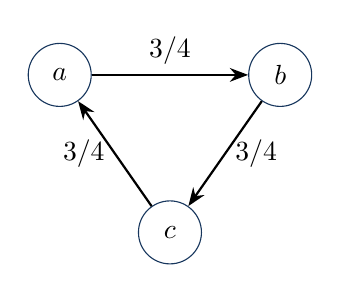
\begin{tikzpicture}[>=Stealth, every node/.style={font=\normalsize}]
\node[circle,draw=courseblue,minimum size=8mm] (a) at (0,1.5) {$a$};
\node[circle,draw=courseblue,minimum size=8mm] (b) at (2.8,1.5) {$b$};
\node[circle,draw=courseblue,minimum size=8mm] (c) at (1.4,-.5) {$c$};
\draw[->,thick] (a) -- node[above] {$3/4$} (b);
\draw[->,thick] (b) -- node[right] {$3/4$} (c);
\draw[->,thick] (c) -- node[left] {$3/4$} (a);
\end{tikzpicture}
\caption{An arrow points from the response selected with probability $3/4$
to its competitor. The probabilities remain fixed while the frequencies
with which the three pairs are compared change.}
\label{fig:cycle}
\end{figure}

We vary the frequency of comparing $c$ with $a$. For
$0<\varepsilon\le1/3$, set
\begin{equation}
 \nu_\varepsilon(a,b)=\nu_\varepsilon(b,c)=\frac{1-\varepsilon}{2},
 \qquad \nu_\varepsilon(c,a)=\varepsilon,
 \label{eq:cyclic-design}
\end{equation}
and assign zero mass to the other orientations. The comparison graph
is complete for every allowed $\varepsilon$. Only the relative sampling
frequencies change.

\begin{proposition}[Design-dependent reversal at the population optimum]
\label{prop:design-reversal}
For \cref{eq:true-cycle,eq:cyclic-design}, the population score objective
$L_{\nu_\varepsilon,p}$ has a unique minimizer up to an
additive constant.
Fix the additive constant by setting $r(b)=0$. Then the minimizing scores
have the form $(d_\varepsilon,0,-d_\varepsilon)$.
For $\varepsilon=1/3$, $d_\varepsilon=0$ and every fitted comparison
probability equals $1/2$. For $0<\varepsilon<1/3$,
\begin{equation}
 0<d_\varepsilon<\log3,
 \qquad p_{r_\varepsilon}(c,a)=\sigma(-2d_\varepsilon)<\frac12,
 \label{eq:design-reversal}
\end{equation}
even though the true probability $p(c,a)$ equals $3/4$.
\end{proposition}

\Cref{ex:l19-design-reversal} asks you to prove the proposition by using
strict convexity to reduce the fit to one score margin, then locating the
minimum of the resulting scalar loss. The score differences must sum to
zero around the cycle. Fitting positive margins on $(a,b)$ and $(b,c)$
therefore forces a negative margin on $(c,a)$. When the last comparison
has smaller weight, the fitting procedure improves the first two fits at
its expense. The exercise also asks how far the reversal can go as that
weight tends to zero.
The failure persists at the population optimum; it does not require
missing pairs, finite-sample noise, or incomplete optimization.

Evaluator heterogeneity can create another source of incompatibility.
Each evaluator may individually follow a scalar logistic model, while
the probabilities pooled across evaluators fail every scalar logistic
representation. \Cref{ex:l19-pooled-evaluators} asks you to verify this
possibility with three finite score vectors. The population being averaged
is therefore part of the preference-learning problem.

\section{Choosing a policy from reward differences}
\label{sec:gibbs}

Suppose a score function $r$ has been specified. A score difference says
which response has higher reward, but does not by itself specify how
often a generator should produce either response. We now choose a decision
objective that balances reward against deviation from a reference policy.

Let $\pi_{\rm ref}(y)>0$ for every $y\in\cY$, and choose $\beta>0$.
The \emph{KL-regularized reward objective} is
\begin{equation}
 F_r(\pi)=\sum_{y\in\cY}\pi(y)r(y)-\beta\KL(\pi,\pi_{\rm ref}),
 \qquad \pi\in\Delta_{\cY},
 \label{eq:reward-objective}
\end{equation}
where the course notation for KL divergence is
\[
 \KL(\pi,q)=\sum_{y\in\cY}\pi(y)\log\frac{\pi(y)}{q(y)}.
\]
Terms with $\pi(y)=0$ contribute zero. Positive reference mass makes
\cref{eq:reward-objective} finite for every policy. The reward term favors
responses with high scores; the penalty charges for changing probabilities
relative to the reference. The comparison probabilities alone specify
neither $\pi_{\rm ref}$ nor $\beta$.
\endnote{\textbf{Reference support.} If the reference assigns zero mass
to some responses, a policy with positive mass there has infinite KL
divergence. The finite-objective optimization can instead be carried out
on the reference support. The full-support assumption in the main text
makes that support restriction explicit through the choice of $\cY$.}
\label{en:reference-support}

\begin{theorem}[Gibbs optimizer and exact objective gap]
\label{thm:gibbs}
For finite $\cY$, finite $r$, positive $\pi_{\rm ref}$, and $\beta>0$,
define
\begin{equation}
 Z_r=\sum_y\pi_{\rm ref}(y)e^{r(y)/\beta},\qquad
 \pi_r^\star(y)=\frac{\pi_{\rm ref}(y)e^{r(y)/\beta}}{Z_r}.
 \label{eq:gibbs-policy}
\end{equation}
The distribution $\pi_r^\star$ is the unique maximizer of $F_r$ on
$\Delta_{\cY}$. For every $\pi\in\Delta_{\cY}$,
\begin{equation}
 F_r(\pi)=\beta\log Z_r-\beta\KL(\pi,\pi_r^\star),\qquad
 F_r(\pi_r^\star)-F_r(\pi)=\beta\KL(\pi,\pi_r^\star).
 \label{eq:gibbs-gap}
\end{equation}
\end{theorem}

\begin{proof}
The finite sum $Z_r$ is positive, so \cref{eq:gibbs-policy} defines a
strictly positive probability distribution. For every $y$,
\[
 \log\frac{\pi_r^\star(y)}{\pi_{\rm ref}(y)}
 =\frac{r(y)}{\beta}-\log Z_r.
\]
Using the zero-mass convention when needed, expand
\begin{align*}
 \beta\KL(\pi,\pi_r^\star)
 &=\beta\sum_y\pi(y)\log\frac{\pi(y)}{\pi_{\rm ref}(y)}
   -\beta\sum_y\pi(y)\log\frac{\pi_r^\star(y)}{\pi_{\rm ref}(y)}\\
 &=\beta\KL(\pi,\pi_{\rm ref})-\sum_y\pi(y)r(y)+\beta\log Z_r.
\end{align*}
Rearranging gives the first identity. KL divergence is nonnegative and
vanishes exactly when its two distributions agree. Hence $\pi_r^\star$
is the unique maximizer, with value $\beta\log Z_r$, and subtraction
gives the objective-gap identity.
\end{proof}

The objective-gap identity lets us compare candidate policies by a KL
divergence from the Gibbs policy. We will use that comparison in
\cref{sec:restricted} to distinguish reward optimization from preference
fitting when the policy class is restricted.

The optimizer is called a \emph{Gibbs policy}: it reweights the reference
by exponentiated reward. Its odds obey
\begin{equation}
 \frac{\pi_r^\star(y)}{\pi_r^\star(y')}
 =\frac{\pi_{\rm ref}(y)}{\pi_{\rm ref}(y')}
   \exp\!\left(\frac{r(y)-r(y')}{\beta}\right).
 \label{eq:gibbs-odds}
\end{equation}
Thus reward differences are exactly the score information needed for this
decision rule. Adding a constant to all rewards changes the optimal value
but leaves the policy unchanged. Scaling rewards at fixed $\beta$ changes
the policy in general; scaling both rewards and $\beta$ by the same
positive factor preserves \cref{eq:gibbs-odds}.

We can now combine score identification with the Gibbs formula.

\begin{corollary}[Connected comparisons identify the optimal policy]
\label{cor:policy-identification}
Suppose $G_\nu$ is connected and $p_r(y,y')=p(y,y')$ whenever
$\nu(y,y')>0$, for a score function $r:\cY\to\R$. Fix
$\pi_{\rm ref}\in\Delta_{\cY}$ with $\pi_{\rm ref}(y)>0$ for every $y$
and fix $\beta>0$. Then the population preference probabilities on the
observed pairs uniquely determine the maximizer $\pi_r^\star$ of $F_r$.
More precisely, every $s:\cY\to\R$ with $p_s=p$ on those pairs satisfies
$\pi_s^\star=\pi_r^\star$.
\end{corollary}

\begin{proof}
By \cref{prop:identification}, every such $s$ satisfies $s=r+c$ for a
constant $c\in\R$. Hence $Z_s=e^{c/\beta}Z_r$, and the common factor
$e^{c/\beta}$ cancels in \cref{eq:gibbs-policy}, giving
$\pi_s^\star=\pi_r^\star$.
\end{proof}

Thus it suffices that the positive-probability comparisons connect all
responses. For example, on $\cY=\{a,b,c\}$ the support
$\operatorname{supp}(\nu)=\{(a,b),(b,c)\}$ forms a connected path;
the pair $(a,c)$ need not be observed. \Cref{ex:l19-three-response-comparisons}(b)
asks you to recover the scores and Gibbs policy from probabilities on this
path. The reference and penalty determine how the identified score
differences affect sampling.

Correct specification is essential to \cref{cor:policy-identification}.
For misspecified comparisons, the fitted score
$\widehat r$ still defines a Gibbs policy, but that policy optimizes
$F_{\widehat r}$. The fitted policy's interpretation inherits the compromise made when
fitting $\widehat r$.

\section{Direct preference optimization}
\label{sec:dpo}

The Gibbs formula describes the optimum for a supplied reward. Enumerating
all responses to compute its normalization is generally impractical for a
language model. We can instead express reward differences through a
policy's log probabilities and fit the preference observations directly.
The resulting objective is still a binary log loss, now parameterized by
the policy.

\subsection{Replacing score differences by policy log ratios}

For every strictly positive policy $\pi$, define its \emph{implicit reward}
and predicted comparison probabilities by
\begin{equation}
 r_\pi(y)=\beta\log\frac{\pi(y)}{\pi_{\rm ref}(y)},\qquad
 q_\pi(y,y')=\sigma(r_\pi(y)-r_\pi(y')).
 \label{eq:implicit-reward}
\end{equation}
For the Gibbs policy, \cref{eq:gibbs-policy} gives
\begin{equation}
 r_{\pi_r^\star}(y)=r(y)-\beta\log Z_r,
 \qquad q_{\pi_r^\star}(y,y')=p_r(y,y').
 \label{eq:inverse-gibbs}
\end{equation}
The normalizing term cancels in each difference. Conversely, the Gibbs
policy for $r_\pi$ is $\pi$, with $Z_{r_\pi}=1$; see
\cref{ex:l19-dpo-algebra}(a). Thus finite score functions modulo a common constant
correspond to strictly positive policies, for the fixed reference and penalty.
The algebraic correspondence holds even when the observed preferences are
misspecified.

For a general policy $\pi\in\Delta_{\cY}$, extend the comparison
probabilities by
\[
 q_\pi(y,y')=
 \frac{(\pi(y)/\pi_{\rm ref}(y))^\beta}
 {(\pi(y)/\pi_{\rm ref}(y))^\beta+(\pi(y')/\pi_{\rm ref}(y'))^\beta}
 \qquad\text{when }\pi(y)+\pi(y')>0.
\]
Use the convention $q_\pi(y,y')=1/2$ when both policy probabilities are
zero. The resulting function $q_\pi\in\cQ$ agrees with
\cref{eq:implicit-reward} for strictly positive policies. The corresponding
logistic expression in the two policy log ratios is valid whenever
$\pi(y),\pi(y')>0$, even if other policy probabilities are zero.
\Cref{ex:l19-dpo-algebra}(b) asks you to verify this pairwise identity
and the reversal identity $q_\pi(y',y)=1-q_\pi(y,y')$.

For the independent triples of \cref{eq:experiment}, the empirical
\emph{direct preference optimization loss} is
\begin{equation}
 L_{{\rm DPO},n}(\pi)
 =-\frac1n\sum_{i=1}^n\bigl[
 C_i\log q_\pi(Y_i,Y_i')+(1-C_i)\log(1-q_\pi(Y_i,Y_i'))\bigr].
 \label{eq:empirical-dpo}
\end{equation}
Reorder each observed pair so that $Y_i^+$ is selected and $Y_i^-$ is
rejected. The label for the reordered pair is $C_i^+=1$ by definition,
so its binary log loss is $-\log q_\pi(Y_i^+,Y_i^-)$. For a strictly
positive policy, substituting \cref{eq:implicit-reward} gives
\begin{equation}
 L_{{\rm DPO},n}(\pi)
 =-\frac1n\sum_{i=1}^n\log\sigma\!\left(
 \beta\log\frac{\pi(Y_i^+)}{\pi_{\rm ref}(Y_i^+)}
 -\beta\log\frac{\pi(Y_i^-)}{\pi_{\rm ref}(Y_i^-)}\right).
 \label{eq:winner-dpo}
\end{equation}
The selected response is the one chosen in that observation. For stochastic
preferences, repeated comparisons can select different responses.
\Cref{ex:l19-dpo-algebra}(c) asks you to check the equality of the two
empirical loss expressions for both possible labels.

\subsection{When population DPO identifies the regularized optimum}

We next connect comparison fitting to the decision objective. The
population DPO loss is the same preference loss parameterized by the policy:
\[
 L_{\rm DPO}:\Delta_{\cY}\to[0,\infty],\qquad
 L_{\rm DPO}(\pi):=L_{\nu,p}(q_\pi).
\]
The relevant \emph{policy realizability} condition is that the available class contains
$\pi_r^\star$, the Gibbs policy for the true preference score.

\begin{theorem}[Population DPO identification]
\label{thm:dpo}
Suppose $p=p_r$ on the observed pairs for a finite score function $r$,
the comparison graph is connected on $\cY$, $\pi_{\rm ref}>0$, and
$\beta>0$. Let $\Pi\subseteq\Delta_{\cY}$ be a policy class containing
$\pi_r^\star$. Then $\pi_r^\star$ is the unique minimizer of
$L_{\rm DPO}$ over $\Pi$. More precisely, for every $\pi\in\Pi$,
\begin{equation}
 L_{\rm DPO}(\pi)-L_{\rm DPO}(\pi_r^\star)
 =\E\!\left[\KL\!\left(
 \operatorname{Bernoulli}(p_r(Y,Y')),
 \operatorname{Bernoulli}(q_\pi(Y,Y'))\right)\right].
 \label{eq:dpo-regret}
\end{equation}
The expectation uses the pair drawn from $\nu$ in the comparison experiment.
\end{theorem}

\begin{proof}
By \cref{eq:inverse-gibbs}, $q_{\pi_r^\star}=p_r=p$ on the observed
pairs. Substituting $q=q_\pi$ in \cref{eq:reward-regret} gives
\cref{eq:dpo-regret}. Nonnegativity of KL divergence shows that
$\pi_r^\star$ minimizes $L_{\rm DPO}$ over $\Pi$. Its loss is the
expected binary entropy, bounded above by $\log 2$.

Let $\pi\in\Pi$ be a minimizer. By \cref{eq:dpo-regret},
$q_\pi=p_r=q_{\pi_r^\star}$ on every pair with positive $\nu$ mass.
The definitions of $q_\pi$ and $\pi_r^\star$ therefore give
\[
 \frac{\pi(y)}{\pi_r^\star(y)}
 =\frac{\pi(y')}{\pi_r^\star(y')}
\]
on every observed edge. Connectedness makes this ratio constant across
$\cY$, so $\pi=c\pi_r^\star$ for some $c\ge0$. Both policies sum to
one, hence $c=1$ and $\pi=\pi_r^\star$.
\end{proof}

The population preference loss and the regularized reward objective have
a common optimizer under the theorem's assumptions, but their values and approximation
errors are different. The preference loss measures prediction error on
sampled pairs. The reward objective evaluates the response distribution
produced by the policy. The next section shows that this distinction can
change which policy is selected when the ideal policy is unavailable.

\subsection{What a language-model update computes}

Restore the prompt $u$. A fixed-data DPO update receives a minibatch of
prompt, selected-response, and rejected-response triples, a frozen
reference model, and the current model. The update evaluates both responses
under both models and differentiates the logistic loss in
\cref{eq:winner-dpo} with respect to the current parameters. Reference
log probabilities can be computed once and stored.

For a terminated response $y$ that includes its end-of-sequence decision,
the autoregressive model of Lecture 1 gives
\begin{equation}
 \log\pi_\theta(y\mid u)
 =\sum_{h=1}^{|y|}\log p_\theta(y_h\mid u,y_{<h}).
 \label{eq:sequence-score}
\end{equation}
A fixed maximum response length, with termination forced at the limit,
makes the response set finite. The probability in \cref{eq:sequence-score}
uses the same termination convention. The observed prefixes permit
teacher-forced scoring: the update evaluates the tokens already in the
dataset. Each pair requires scores for two responses and backpropagation
through the current model. The update requests no fresh response or preference
label; acquiring the comparison dataset is a separate cost.%
\endnote{\textbf{Length normalization.} Dividing
\cref{eq:sequence-score} by response length replaces sequence log
probability by a different score. Substituting that score into the loss
changes the objective analyzed in \cref{thm:dpo}.}
\label{en:length}

The parameters $\theta$ are shared across prompts, so an update computed
from one prompt can change the policy's predictions for other prompts.

\section{Restricted policies can change the preferred optimizer}
\label{sec:restricted}

\emph{Policy-class misspecification} occurs here when the available class
$\Pi$ excludes the Gibbs optimizer $\pi_r^\star$. The preference model
itself can remain correct. We compare the best available policy for
population DPO with the best available policy for the true regularized
reward, holding the class fixed for both optimizations.

Take $\cY=\{a,b\}$, a uniform reference, $\beta=1$, and
$r(a)=\log3$, $r(b)=0$. The true preference probability is $p(a,b)=3/4$.
For $q\in(0,1)$, let $\pi_q(a)=q$ and $\pi_q(b)=1-q$. The ideal
policy is $\pi_{3/4}$. For a candidate $\pi_q$, the DPO comparison
prediction simplifies to
\begin{equation}
 q_{\pi_q}(a,b)=\sigma\!\left(\log\frac{q}{1-q}\right)=q.
 \label{eq:binary-dpo}
\end{equation}
Write $\mathrm{kl}(v,w)=v\log(v/w)+(1-v)\log((1-v)/(1-w))$ for
binary KL divergence. The two preceding theorems give
\begin{equation}
 L_{\rm DPO}(\pi_q)-L_{\rm DPO}(\pi_{3/4})=\mathrm{kl}(3/4,q),
 \qquad
 F_r(\pi_{3/4})-F_r(\pi_q)=\mathrm{kl}(q,3/4).
 \label{eq:opposite-kl}
\end{equation}
Both gaps vanish at the ideal policy. Away from that policy, their
opposite KL directions can order the candidates differently.

\begin{proposition}[Different optima in the same restricted class]
\label{prop:restricted}
In the two-response setting above, restrict the class to
$\Pi=\{\pi_{11/20},\pi_{9/10}\}$. Population DPO uniquely selects
$\pi_{11/20}$, while $F_r$ is uniquely maximized over $\Pi$ by
$\pi_{9/10}$.
\end{proposition}

\Cref{ex:l19-restricted-policies} asks you to prove the proposition by
evaluating the two KL gaps in \cref{eq:opposite-kl}. The exact gap
identities make this comparison possible: each objective measures a
different divergence from the same ideal policy.

The construction has a correct Bradley--Terry preference model, complete comparison
coverage, and exact population optimization. Only policy realizability
fails. A common optimum over all distributions therefore does not imply
a common optimum in an arbitrary restricted class. The example establishes
the possibility of different selections; it does not quantify their
prevalence or magnitude for trained language models.

The reward/policy reparameterization in \cref{eq:implicit-reward} remains
valid. Fitting an implicit reward $r_\pi$ still makes $\pi$ the Gibbs
optimizer of that fitted reward. \Cref{prop:restricted} compares a different
pair of operations: fitting comparisons within $\Pi$ and directly optimizing
the true $F_r$ within that same $\Pi$. A reward fitted under a restriction
need not preserve the ordering of available policies under the true reward.

More generally, a class $\Pi$ of strictly positive policies induces the
implicit reward class
$\cR_\Pi=\{r_\pi:\pi\in\Pi\}$. The binary-KL identity in
\cref{eq:dpo-regret} holds for each positive policy even when $\pi_r^\star$
is excluded from $\Pi$. DPO therefore chooses a fit within $\cR_\Pi$ using
comparison errors weighted by $\nu$. If the true score differences cannot
be represented in $\cR_\Pi$, the weights determine the approximation problem.
This is another source of dependence on the comparison design: the
preferences may satisfy Bradley--Terry while the policy-induced reward
class is too restrictive. In \cref{prop:design-reversal}, by contrast,
the probabilities have no Bradley--Terry representation.

\section{Missing comparisons and finite-data limitations}
\label{sec:coverage}

The preceding failures came from incompatible model or policy restrictions.
The observations can also leave parts of behavior unidentified even when
the Bradley--Terry model is correct. We first remove comparisons, then distinguish
that information problem from the limitations of finite samples.

\subsection{A response with unconstrained probability}

Return to three responses, a uniform reference, and $\beta=1$, but suppose
only $(a,b)$ is compared, with $p(a,b)=3/4$. For every $t>0$, define
\begin{equation}
 (\pi_t(a),\pi_t(b),\pi_t(c))=\frac{(3,1,t)}{4+t}.
 \label{eq:unidentified-policy}
\end{equation}
Every policy in this family has $q_{\pi_t}(a,b)=3/4$, so each attains the
minimum population comparison loss, while $\pi_t(c)$ ranges over $(0,1)$.
\Cref{ex:l19-unobserved-responses}(a) asks you to verify these claims.
An unseen response can receive
almost any probability without changing the optimal observed preference
fit. The componentwise constants of \cref{prop:identification} become
undetermined relative masses across graph components.

For any fixed complete Bradley--Terry target extending the observed
probability, the regularized reward objective has one Gibbs optimizer.
The comparison data do not identify which member of the displayed family
it is. An optimizer or parameterization may choose a member, but that choice
uses information or preferences beyond the observed comparison probabilities.

\subsection{A better comparison fit can reduce both response probabilities}
\label{sec:displacement}

An improvement in a probability ratio need not increase either probability.
\emph{Likelihood displacement} describes a growing log-probability margin
between a preferred and a rejected response while the probabilities of both
responses fall. The missing comparisons above permit a finite example even
at the population level.

\begin{example}[Improved comparison fit with less mass on the preferred response]
\label{ex:displacement}
Keep the uniform reference, $\beta=1$, and the single observed pair $(a,b)$
with $p(a,b)=3/4$. Consider two policies, listed in the order $(a,b,c)$:
\[
 \pi^{\rm old}=(0.6,0.3,0.1),\qquad
 \pi^{\rm new}=(0.3,0.1,0.6).
\]
The population losses satisfy
\[
 L_{\rm DPO}(\pi^{\rm new})<L_{\rm DPO}(\pi^{\rm old}).
\]
Thus the population preference fit improves, although the probability of
the majority-preferred response $a$ falls from $0.6$ to $0.3$ and that of
$b$ falls from $0.3$ to $0.1$. Response $b$ loses a larger proportion of
its probability than $a$, so $\pi(a)/\pi(b)$ increases while their combined
mass decreases. The unobserved response $c$ receives the remaining mass.
\Cref{ex:l19-unobserved-responses}(b) asks you to establish the loss
inequality using the binary-KL identity from \cref{prop:population-recovery}.
\end{example}

The example compares two policies; it does not assert that gradient training
follows this change. Training dynamics and the model's parameterization
determine which probabilities actually increase. Nor does a decrease in
the probability of one preferred response alone imply worse behavior:
the responses receiving that mass may be equally good or better. Judgments
comparing $c$ with $a$ or $b$ are absent here. This information limitation
is distinct from both cyclic preferences and a restricted policy class.

\subsection{Positive coverage does not specify a sample size}

Connectedness is qualitative. Let $e$ be an edge whose removal disconnects
the population comparison graph. Suppose
$\delta=\P(\{Y,Y'\}=e)>0$. For $n$ independent comparisons,
\begin{equation}
 \P\!\left(\{Y_i,Y_i'\}\ne e\text{ for all }i=1,\ldots,n\right)
 =(1-\delta)^n.
 \label{eq:rare-edge}
\end{equation}
On this event, the sample comparison graph is disconnected. Adding separate
constants to the scores in its components leaves every observed comparison
prediction, and hence the empirical loss, unchanged. For any fixed $n$,
the probability of this event tends to one as $\delta\downarrow0$.
Thus connected population support alone does not ensure that a finite
dataset identifies score differences between all response groups. A small
prediction loss averaged under $\nu$ is a different requirement: the
rare comparisons receive correspondingly little weight in that average.
\Cref{ex:l19-rare-comparisons} asks you to derive the probability and
show how missing the edge leaves relative score offsets unidentified.

Even with two responses and every observation on their single connecting
edge, all sampled labels can agree. An unconstrained logistic fit then
approaches probability one for the selected response and has no finite
optimal margin. \Cref{ex:l19-unanimous-comparisons} asks you to derive
this boundary behavior and its probability under stochastic labels.
The phenomenon is the same nonattainment seen for separable log-loss
problems in Lectures 10--11.

The distinction from Lecture 18 is the observation being acquired.
Teacher demonstrations reveal behavior; preference queries reveal judgments
on chosen pairs. Changing the query process can add previously absent
information. Under misspecification, changing that process can also change
the best-fitting compromise, as \cref{prop:design-reversal} shows.

After fitting a reward, policy optimization can concentrate on responses
that were rare in the comparison data. The next lecture asks when errors
of the learned reward remain controlled under that new distribution.
The present results identify why a well-defined fitting objective and a
population optimizer alone do not settle that reliability question.

\section{Take-home messages}
\label{sec:take-home}

\begin{itemize}[leftmargin=*]
\item Under the Bradley--Terry model, connected comparisons identify scores
up to an additive constant. Population log-loss minimization recovers those
scores after fixing the constant. Cycle restrictions can fail even when all
majority comparisons admit a consistent ranking.
\item When Bradley--Terry scores cannot represent the preferences, the comparison
design affects the population fit. Reweighting fixed cyclic preferences can reverse a
fitted majority comparison while every pair remains observed.
\item A reference policy and a positive KL penalty convert reward differences
into a unique Gibbs policy. For any policy $\pi$, the gap from the optimum is
$\beta\KL(\pi,\pi_r^\star)$.
\item Population DPO recovers that policy under preference-model correctness,
connected comparisons, and policy realizability. Restricting the policy
class can make better comparison likelihood correspond to worse regularized
reward, even with exact probabilities and exact optimization.
\item Missing comparisons, rare comparisons, finite-sample nonattainment,
and misspecification are distinct limitations. Their remedies depend on
whether the problem is absent information, statistical uncertainty, or
incompatible modeling assumptions.
An improved comparison fit can lower the probabilities of both compared
responses while unobserved responses gain mass.
\end{itemize}

\printendnotes

\section*{Bibliographical notes}
\label{sec:bibliographical-notes}

\paragraph{Use in language-model post-training.}
The terminology recalled in the opening is defined in Lecture 1;
Lecture 18 identifies the SFT objective with teacher-forced behavior cloning.
The \citet{llama2024} report, Section 4, documents repeated SFT and DPO
stages, with preference-trained reward models also used to select responses
for SFT. Their DPO implementation includes a chosen-response likelihood
term and masks formatting tokens. Thus the report supports use of DPO,
while the deployed loss differs from our basic formula.
\citet{ai2olmo2025} documents the SFT--DPO--verifiable-reward RL sequence
for Olmo 3-Think. These are examples of adoption, not estimates of an
industry-wide usage rate.

\paragraph{Bradley--Terry identification.}

\citet{bradley1952} introduced the paired-comparison model used here.
In \cref{prop:identification,prop:cycles}, logits are expressed as differences
of vertex scores. The path and cycle
proofs are provided in these notes. The distinction between ordinal rankings
and the cardinal gaps specified by a fixed logistic model is essential
to interpreting that identification claim.
\Cref{prop:population-recovery} combines graph identification with the
binary log-loss regret identity from Lecture 3 to establish recovery by
population maximum likelihood.

\paragraph{Broader preference models.}
\citet{bengs2022}, Section 2, presents linear stochastic transitivity
models and their relation to additive random utility, including logistic
and probit links. \citet{shah2016}, Section 2, studies the broader class
of strongly stochastically transitive comparisons. \Cref{app:preference-models}
uses these distinctions to separate identification under a known link
from assumptions that specify only an ordering.

\citet{noothigattu2020} studies axioms of maximum-likelihood learning from
pairwise comparisons. For the model classes covered by their theorems,
the fitted rules satisfy Pareto efficiency and monotonicity, while other
consistency requirements, including agreement with majority opinion, can
fail. These results concern properties of the fitted rule; they are
different questions from whether the observed probabilities admit a
Bradley--Terry representation. Their discussion also motivates distinguishing
individual evaluator models from pooled comparisons.

The triangle bounds in \cref{ex:l19-random-utility-cycles} are classical
necessary restrictions on binary probabilities induced by random rankings.
\citet{sprumont2022} gives further background and distinguishes these
restrictions from a full characterization of random utility models.
The exercise asks for a direct proof and finite constructions.

\paragraph{The ideal population objective and its limitations.}

The Gibbs policy, reward/policy change of variables, and DPO loss follow
\citet{rafailov2023}, Sections 3--5 and Appendices A.1--A.2. The exact
objective-gap identity is the KL calculation underlying their optimizer.
\Cref{thm:dpo} combines that change of variables with binary log-loss
properness and makes graph connectivity and policy realizability explicit.
The result concerns a shared population optimizer under the stated
assumptions. The paper's language-model experiments are separate evidence
from this identification argument.

\Cref{prop:design-reversal,prop:restricted} are elementary counterexamples
worked out for these notes; no claim of novelty is intended. The first
shows how the sampling design determines a misspecified population fit.
The second uses opposite KL directions to distinguish approximation under
two criteria with the same unrestricted optimum. Neither example estimates
the frequency of such failures in practical post-training. The pooled
evaluator exercise gives a further finite example of model incompatibility.
The Bradley--Terry model and its population projection connect to the earlier
misspecification discussion in Lecture 7; finite-sample nonattainment
connects to the logistic examples in Lectures 10--11.

\paragraph{Misspecification under policy restrictions.}
\citet{gopalan2026}, Proposition 1, expresses population DPO as a
comparison-weighted binary-KL projection onto policy-induced rewards.
Their Proposition 3 gives a three-response, one-parameter softmax example
with preference reversal and reward decrease, in their sufficiently large
$\beta$ regime. The closest connection is \cref{sec:restricted}:
correct Bradley--Terry preferences can still be incompatible with the
implicit reward class. Our two-policy construction gives an exact global
comparison of the two objectives. Our cyclic example instead violates
Bradley--Terry itself. The distinction matters when identifying which
assumption has failed.

\paragraph{Likelihood displacement and unseen responses.}
\citet{razin2025}, Sections 3--6, studies likelihood displacement and its
dependence on model embeddings and gradient dynamics. In a controlled
experiment, preferring \texttt{No} to \texttt{Never} can increase the
probability of \texttt{Yes}. Their refusal-training experiments also show
that preference updates can reduce refusal rates. \Cref{ex:displacement}
illustrates the objective's freedom to transfer mass to unobserved responses;
it does not derive the paper's training dynamics. Their theory concerns
instantaneous changes under an idealized feature model. A decrease in one
response's probability alone does not establish worse behavior; the
responses gaining mass must also be evaluated.

\citet{rafailov2024overoptimization}, Sections 3--4, reports deterioration
in GPT-4-judged win rates during direct preference training, including DPO,
and analyzes how incomplete comparisons leave response probabilities
underdetermined. \Cref{eq:unidentified-policy} gives an elementary instance
of this freedom, using strictly positive policies throughout. The empirical
metric is an external model judge, not a known true reward. Neither the
graph example nor the restricted-policy example identifies the cause of
each empirical deterioration.

\Needspace{4\baselineskip}
\paragraph{Reward error and the meaning of the feedback.}
\citet{gao2023} studies reward overoptimization: optimizing a learned proxy
can eventually reduce the score assigned by a separate evaluator. Their
experiments use a larger ``gold'' reward model to supply synthetic
preferences, rather than measuring human judgments throughout optimization.
This is evidence about proxy error under optimization and motivates Lecture
20. The restriction in \cref{prop:restricted} creates a different failure,
even with exact preference probabilities and a known true reward.

\citet{sharma2024}, Section 4, finds that human judgments and preference
models can favor agreement with a user's mistaken beliefs; some forms of
this \emph{sycophancy} increase during their RL experiments. Other forms do
not, and sycophancy is already present before RL. The connection to
\cref{sec:comparisons} is the distinction between predicting judgments and
producing correct responses. A preference target can favor undesirable
behavior even when its statistical model is correctly specified.

\Needspace{12\baselineskip}
\section*{Glossary}

\begin{description}[style=nextline,leftmargin=1.5em,labelindent=0pt]
\item[Fine-tuning and post-training]
Fine-tuning continues parameter training from a checkpoint. Post-training
is the stage after pretraining; SFT, preference fitting, and reward-based
RL are possible components.
\item[Comparison design $\nu$]
The joint probability mass function $\nu\in\Delta_{\cY^2}$ of the response
pair $(Y,Y')$, with $\nu(y,y)=0$ for every $y\in\cY$.
\item[Preference probability $p(y,y')$]
The evaluator population's probability of selecting $y$ when compared with $y'$.
\item[Random utility model]
A common joint law of utilities $(U_y)_{y\in\cY}$, independent of the
presented pair, gives $p(y,y')=\P(U_y>U_{y'})$. We assume zero tie probability.
\item[Additive random utility model]
Utilities have the form $U_y=r(y)+\varepsilon_y$, with a deterministic
score function and a specified joint perturbation law.
\item[Bradley--Terry model]
The logistic representation $p_r(y,y')=\sigma(r(y)-r(y'))$, obtained
from additive independent standard Gumbel perturbations.
\item[Majority ordering]
A strict total order $\succ$ satisfying
$y\succ y'\Longleftrightarrow p(y,y')>1/2$ for distinct responses.
\item[Linear stochastic transitivity and probit comparisons]
The common-link representation $p(y,y')=F(r(y)-r(y'))$ from
\cref{app:preference-models}. The choice $F=\Phi$, the standard normal
distribution function, gives the Thurstone--Mosteller probit model.
\item[Strong stochastic transitivity]
An ordering under which a higher-ranked response is at least as likely
to defeat every other response; see \cref{def:strong-stochastic-transitivity}.
\item[Comparison graph]
The undirected graph joining pairs with positive comparison probability.
Connected components determine which score differences can be identified.
\item[Logit and cycle compatibility]
The logit is $\log(v/(1-v))$. A scalar logistic representation requires
its sum around every oriented comparison cycle to vanish.
\item[Preference-model misspecification]
No score function in the specified preference model reproduces all
observed-pair probabilities.
\item[Population preference loss $L_{\nu,p}$]
The expected binary log loss of comparison predictions $q$. For a score
function $r$, the notation $L_{\nu,p}(r)$ means $L_{\nu,p}(p_r)$.
\item[Reference policy and KL penalty]
The distribution $\pi_{\rm ref}$ and coefficient $\beta>0$ defining
the cost of changing the policy in $F_r$.
\item[Gibbs policy]
The distribution proportional to $\pi_{\rm ref}(y)e^{r(y)/\beta}$,
which uniquely maximizes $F_r$ over all response distributions.
\item[Implicit reward]
For a strictly positive policy $\pi$, the score
$r_\pi=\beta\log(\pi/\pi_{\rm ref})$ whose Gibbs policy is $\pi$.
\item[Direct preference optimization (DPO)]
Preference-likelihood fitting through policy-induced comparison predictions:
$L_{\rm DPO}(\pi)=L_{\nu,p}(q_\pi)$.
\item[Policy realizability and policy-class misspecification]
Whether the available policy class contains the Gibbs optimizer of the true
preference score. This condition differs from whether Bradley--Terry scores
represent the preference probabilities.
\item[Likelihood displacement]
The log-probability margin between a preferred and a rejected response
increases while both response probabilities decrease.
\end{description}

\Needspace{17\baselineskip}
\section{Exercises}
\label{sec:exercises}

\exerciseinstructions
\setcounter{courseexercise}{0}
\Needspace{17\baselineskip}
\begin{exercisechunk}
\item \textbf{Gumbel utilities and Bradley--Terry probabilities.}
\label[exercise]{ex:l19-gumbel-comparisons}
\exerciseprofile{2}{1}{2}{\excalculation}{%
Derive a comparison link from an additive utility model.}
Let $\cY$ be a finite response set and fix $r:\cY\to\R$.
Let $(\varepsilon_y)_{y\in\cY}$ be mutually independent random variables
with distribution function $G:\R\to(0,1)$,
$G(t)=\exp(-e^{-t})$. Set $U_y=r(y)+\varepsilon_y$.
Show that, for distinct $y,y'\in\cY$,
\[
 \P(U_y>U_{y'})
 =\frac{e^{r(y)}}{e^{r(y)}+e^{r(y')}}
 =\sigma(r(y)-r(y')),
 \qquad \sigma(z)=\frac{1}{1+e^{-z}}.
\]
\begin{hints}
Condition on one of the two perturbations.
\end{hints}
\end{exercisechunk}

\Needspace{25\baselineskip}
\begin{exercisechunk}
\item \textbf{Identification with a known comparison link.}\suppmark
\label[exercise]{ex:l19-general-link}
\exerciseprofile{2}{2}{2}{\exproof\quad\exinterpretation}{%
Determine how knowledge of the comparison link affects score identification.}
Let $G=(\cY,E)$ be a finite undirected graph, and let
$F:\R\to(0,1)$ be a known strictly increasing bijection satisfying
$F(-t)=1-F(t)$. Assign a probability $p(y,y')\in(0,1)$ to each oriented
edge, with $p(y',y)=1-p(y,y')$. Consider score functions
$r:\cY\to\R$ and predictions $p_r^F(y,y')=F(r(y)-r(y'))$.
\begin{enumerate}[(a)]
\item Show that $p_r^F=p_s^F$ on all edges if and only if $r-s$ is
constant on each connected component of $G$.
\item Show that a score function satisfying $p=p_r^F$ on all edges exists
if and only if every oriented cycle $y_0,\ldots,y_m=y_0$ satisfies
\[
 \sum_{j=0}^{m-1}F^{-1}(p(y_j,y_{j+1}))=0.
\]
\item Now allow the link to be unknown. For $a>0$, define
$F_a(t)=F(t/a)$ and $r_a(y)=ar(y)$. Show that $(F_a,r_a)$ gives the same
comparison probabilities as $(F,r)$. For a nonconstant $r$, a strictly
positive reference policy $\pi_{\rm ref}$, and a fixed $\beta>0$, show
that the Gibbs policies $\pi_{r_a}^\star$ and $\pi_r^\star$ differ when
$a\ne1$. Explain why identifying comparison probabilities then fails to
identify the Gibbs policy at that fixed $\beta$.
\end{enumerate}
\begin{hints}
For (b), adapt the construction in \cref{app:cycles}.
\end{hints}
\end{exercisechunk}

\Needspace{21\baselineskip}
\begin{exercisechunk}
\item \textbf{Three responses: compatibility and policy identification.}
\label[exercise]{ex:l19-three-response-comparisons}
\exerciseprofile{2}{2}{2}{\exproof\quad\excalculation\quad\exinterpretation}{%
Distinguish checking a preference model from identifying a policy within it.}
Let $\cY=\{a,b,c\}$.  In the Bradley--Terry model, a score function
$r:\cY\to\R$ predicts
\[
 p_r(y,y')=\sigma(r(y)-r(y')),
 \qquad \sigma(z)=\frac{1}{1+e^{-z}}.
\]
\begin{enumerate}[(a)]
\item Set $p(a,b)=p(b,c)=p(a,c)=3/4$, with reverse probabilities $1/4$.
Show that these probabilities admit the majority ordering $a\succ b\succ c$
but have no Bradley--Terry representation. In particular, show that
$p_r(a,b)=p_r(b,c)=3/4$ and $r(b)=0$ force
\[
 (r(a),r(b),r(c))=(\log3,0,-\log3),\qquad p_r(a,c)=9/10.
\]
\item Now suppose the comparison design has support
$\{(a,b),(b,c)\}$ and $p(a,b)=p(b,c)=3/4$. Assume the preference target
satisfies Bradley--Terry; no probability for $(a,c)$ is supplied separately.
For a uniform reference policy and $\beta=1$, the Gibbs policy is
$\pi_r^\star(y)=e^{r(y)}/\sum_{z\in\cY}e^{r(z)}$.
Show that the uniquely identified Gibbs policy is
\[
 (\pi_r^\star(a),\pi_r^\star(b),\pi_r^\star(c))=(9,3,1)/13.
\]
Explain why observing $(a,c)$ is unnecessary for this identification,
and why the two observed probabilities alone cannot test the triangle
compatibility condition.
\end{enumerate}
\end{exercisechunk}

\Needspace{20\baselineskip}
\begin{exercisechunk}
\item \textbf{Comparison frequencies and a reversed preference.}
\label[exercise]{ex:l19-design-reversal}
\exerciseprofile{2}{2}{2}{\exproof\quad\excalculation}{%
Use convexity to identify the global population fit under misspecification.}
For $v\in(0,1)$ and $z\in\R$, let
$\ell_v(z)=\log(1+e^z)-vz$ as in \cref{eq:logistic-loss}.
On $\cY=\{a,b,c\}$, set $p(a,b)=p(b,c)=p(c,a)=3/4$ and use
the reversal rule for the other orientations. For $0<\varepsilon\le1/3$,
let $\nu_\varepsilon(a,b)=\nu_\varepsilon(b,c)=(1-\varepsilon)/2$
and $\nu_\varepsilon(c,a)=\varepsilon$, with zero mass elsewhere.
\begin{enumerate}[(a)]
\item Derive
\[
 \ell_v'(z)=\sigma(z)-v,\qquad
 \ell_v''(z)=\sigma(z)(1-\sigma(z))>0.
\]
Show that $\ell_v(z)\to\infty$ as $|z|\to\infty$ and that its unique
minimizer is $\operatorname{logit}(v)$.
\item Fix $r(b)=0$. Show that minimizing $L_{\nu_\varepsilon,p}(r)$
over score functions is equivalent to minimizing
\[
 f_\varepsilon(d)=(1-\varepsilon)\ell_{3/4}(d)
                  +\varepsilon\ell_{3/4}(-2d),\qquad d\in\R.
\]
Prove that a unique minimizer exists and that the minimizing score vector
has the form $(r(a),r(b),r(c))=(d_\varepsilon,0,-d_\varepsilon)$.
\item Show that
\[
 f_\varepsilon'(0)=\frac{3\varepsilon-1}{4},\qquad
 f_\varepsilon'(\log3)=\frac{13\varepsilon}{10}.
\]
Deduce $d_{1/3}=0$ and, for $0<\varepsilon<1/3$,
$0<d_\varepsilon<\log3$ and
$p_{r_\varepsilon}(c,a)=\sigma(-2d_\varepsilon)<1/2$.
\item \emph{Optional.} Show that $d_\varepsilon\to\log3$ and
$p_{r_\varepsilon}(c,a)\to1/10$ as $\varepsilon\downarrow0$.
For $\varepsilon=1/5$, numerically find the fitted probability to three
decimal places.
\end{enumerate}
\begin{hints}
For (b), write $v=r(a)-r(b)$ and $w=r(b)-r(c)$. Hold $v+w$ fixed
and compare the loss at $(v,w)$ with its value at
$((v+w)/2,(v+w)/2)$.
\end{hints}
\end{exercisechunk}

\Needspace{22\baselineskip}
\begin{exercisechunk}
\item \textbf{Pooling Bradley--Terry evaluators.}
\label[exercise]{ex:l19-pooled-evaluators}
\exerciseprofile{2}{1}{1}{\excalculation\quad\exinterpretation}{%
Show that pooling correctly specified Bradley--Terry evaluators can produce
preferences that no Bradley--Terry model represents.}
Fix a prompt with responses $a,b,c$. For each comparison, draw an evaluator
type $T$ uniformly from $\{1,2,3\}$, independently of the presented pair.
The three types have score vectors
\[
 \begin{pmatrix}r_1(a)&r_1(b)&r_1(c)\\
                 r_2(a)&r_2(b)&r_2(c)\\
                 r_3(a)&r_3(b)&r_3(c)\end{pmatrix}
 =\begin{pmatrix}\log9&\log3&0\\
                 0&\log9&\log3\\
                 \log3&0&\log9\end{pmatrix}.
\]
Conditional on type $T=t$ and the ordered pair $(y,y')$, the evaluator
selects $y$ with probability $\sigma(r_t(y)-r_t(y'))$, where
$\sigma(z)=(1+e^{-z})^{-1}$. The pooled probability averages over the
unobserved evaluator type:
$p(y,y')=\tfrac13\sum_{t=1}^3\sigma(r_t(y)-r_t(y'))$.
\begin{enumerate}[(a)]
\item Show that $p(a,b)=p(b,c)=p(c,a)=8/15$.
\item Show that no scalar Bradley--Terry score function on $\{a,b,c\}$
represents these pooled probabilities. Identify the violated cycle
restriction and explain why correct specification for each evaluator
type does not imply correct specification after the type is omitted.
\end{enumerate}
\end{exercisechunk}

\Needspace{26\baselineskip}
\begin{exercisechunk}
\item \textbf{Majority cycles in random utility models.}\suppmark
\label[exercise]{ex:l19-random-utility-cycles}
\exerciseprofile{2}{2}{2}{\exproof\quad\exconstruction\quad\exinterpretation}{%
Distinguish failure of Bradley--Terry from failure of a general random utility model.}
Let $U=(U_a,U_b,U_c)\in\R^3$ be jointly distributed, with
$\P(U_y=U_{y'})=0$ for distinct $y,y'\in\{a,b,c\}$.
The same utility law is used for every compared pair, independently of
which pair is presented. Define $p(y,y')=\P(U_y>U_{y'})$.
\begin{enumerate}[(a)]
\item Prove the triangle bounds
\[
 1\le p(a,b)+p(b,c)+p(c,a)\le2.
\]
\item Construct a distribution supported on three utility vectors for which
$p(a,b)=p(b,c)=p(c,a)=2/3$. Verify these probabilities and the absence
of ties.
\item Decide whether the probabilities $p(a,b)=p(b,c)=p(c,a)=3/4$
from \cref{sec:misspecification} admit such a random utility model.
Then construct a random utility model for the pooled probabilities
from \cref{ex:l19-pooled-evaluators}. Explain why incompatibility with
Bradley--Terry has different implications in these two examples.
You may use the identity requested in \cref{ex:l19-gumbel-comparisons}.
\end{enumerate}
\end{exercisechunk}

\Needspace{20\baselineskip}
\begin{exercisechunk}
\item \textbf{Policy ratios and the DPO loss.}
\label[exercise]{ex:l19-dpo-algebra}
\exerciseprofile{1}{2}{2}{\exproof\quad\excalculation}{%
Verify the reward--policy correspondence and the preference-likelihood rewrite.}
Fix finite $\cY$, a strictly positive $\pi_{\rm ref}\in\Delta_{\cY}$,
and $\beta>0$. Use the Gibbs policy and normalizer from
\cref{eq:gibbs-policy}, and the comparison predictions $q_\pi$ defined
in \cref{sec:dpo}, including their extension to policies with zeros.
\begin{enumerate}[(a)]
\item For strictly positive $\pi$, define
$r_\pi(y)=\beta\log(\pi(y)/\pi_{\rm ref}(y))$.
Show that $Z_{r_\pi}=1$ and $\pi_{r_\pi}^\star=\pi$.
For a score function $r:\cY\to\R$, also show that
\[
 r_{\pi_r^\star}(y)=r(y)-\beta\log Z_r,
 \qquad q_{\pi_r^\star}(y,y')=p_r(y,y').
\]
\item For arbitrary $\pi\in\Delta_{\cY}$ and a pair with
$\pi(y),\pi(y')>0$, show that
\[
 q_\pi(y,y')=
 \sigma\!\left(\beta\log\frac{\pi(y)}{\pi_{\rm ref}(y)}
              -\beta\log\frac{\pi(y')}{\pi_{\rm ref}(y')}\right).
\]
Show also that $q_\pi(y',y)=1-q_\pi(y,y')$ for every distinct pair,
including pairs with zero policy probabilities.
\item Let $\pi$ be strictly positive and consider the observed triples
$(Y_i,Y_i',C_i)$ from \cref{eq:experiment}. Put
$(Y_i^+,Y_i^-)=(Y_i,Y_i')$ when $C_i=1$, and
$(Y_i^+,Y_i^-)=(Y_i',Y_i)$ when $C_i=0$.
Show, for either label, that
\[
 -C_i\log q_\pi(Y_i,Y_i')-(1-C_i)\log(1-q_\pi(Y_i,Y_i'))
 =-\log q_\pi(Y_i^+,Y_i^-).
\]
Deduce the equality of \cref{eq:empirical-dpo,eq:winner-dpo}.
\end{enumerate}
\end{exercisechunk}

\Needspace{22\baselineskip}
\begin{exercisechunk}
\item \textbf{Opposite KL directions select different policies.}
\label[exercise]{ex:l19-restricted-policies}
\exerciseprofile{2}{2}{2}{\excalculation\quad\exinterpretation}{%
Use objective-gap identities to compare preference fitting and reward optimization.}
Let $\cY=\{a,b\}$, take a uniform reference and $\beta=1$, and set
$r(a)=\log3$, $r(b)=0$, and $p=p_r$. Write
$\pi_q(a)=q$, $\pi_q(b)=1-q$ for $q\in(0,1)$.
Restrict the policy class to $\Pi=\{\pi_{11/20},\pi_{9/10}\}$.
The binary KL divergence is
$\mathrm{kl}(v,w)=v\log(v/w)+(1-v)\log((1-v)/(1-w))$.
\begin{enumerate}[(a)]
\item Derive the exact differences
\[
 \mathrm{kl}(3/4,11/20)-\mathrm{kl}(3/4,9/10)
 =\frac14\log\frac{1296}{1331}<0,
\]
\[
 \mathrm{kl}(11/20,3/4)-\mathrm{kl}(9/10,3/4)
 =\frac1{20}\log\frac{11^{11}}{2^{20}3^{11}}>0.
\]
\item Prove that $L_{\rm DPO}$ is uniquely minimized over $\Pi$ by
$\pi_{11/20}$, whereas $F_r$ is uniquely maximized over $\Pi$ by
$\pi_{9/10}$. Identify the assumption of \cref{thm:dpo} that fails
for this class, and explain why these selections are consistent with both
objectives having the same unrestricted optimizer.
\end{enumerate}
\begin{hints}
For (b), use the two objective gaps in \cref{eq:opposite-kl}.
\end{hints}
\end{exercisechunk}

\Needspace{22\baselineskip}
\begin{exercisechunk}
\item \textbf{Unobserved responses and probability transfer.}
\label[exercise]{ex:l19-unobserved-responses}
\exerciseprofile{2}{2}{2}{\exproof\quad\excalculation\quad\exinterpretation}{%
Determine which policy probabilities a single comparison leaves unconstrained.}
Let $\cY=\{a,b,c\}$, use a uniform reference and $\beta=1$, and suppose
$\nu(a,b)=1$ and $p(a,b)=3/4$. All policy vectors below list coordinates
in the order $(a,b,c)$.
\begin{enumerate}[(a)]
\item For $t>0$, define $\pi_t=(3,1,t)/(4+t)$. Show that
$q_{\pi_t}(a,b)=3/4$ for every $t$ and that every $\pi_t$ minimizes
the population DPO loss over $\Delta_{\cY}$. Show that
$\pi_t(c)=t/(4+t)$ ranges over $(0,1)$ and explain why the observed
preference probability therefore does not identify the probability of $c$.
\item Let $\pi^{\rm old}=(0.6,0.3,0.1)$ and
$\pi^{\rm new}=(0.3,0.1,0.6)$. Show that
$q_{\pi^{\rm old}}(a,b)=2/3$, $q_{\pi^{\rm new}}(a,b)=3/4$, and
\[
 L_{\rm DPO}(\pi^{\rm old})-L_{\rm DPO}(\pi^{\rm new})
 =\mathrm{kl}(3/4,2/3)>0,
\]
where $\mathrm{kl}$ is binary KL divergence.
Explain how the comparison fit improves while the probabilities of both
$a$ and $b$ decrease, identifying the changed probability ratio and the
response that receives the transferred probability mass.
\end{enumerate}
\begin{hints}
Apply the binary log-loss identity from \cref{prop:population-recovery}
to the single observed pair; no assumption on unobserved preferences is needed.
\end{hints}
\end{exercisechunk}

\Needspace{17\baselineskip}
\begin{exercisechunk}
\item \textbf{A rare comparison connecting two response groups.}
\label[exercise]{ex:l19-rare-comparisons}
\exerciseprofile{2}{1}{1}{\exproof\quad\excalculation\quad\exinterpretation}{%
Distinguish connected population support from comparison coverage in a sample.}
Let $G_\nu$ be connected, and let $e$ be an edge whose removal disconnects
$G_\nu$. Draw $n\ge1$ independent comparisons with pair law $\nu$.
Set $\delta=\P(\{Y,Y'\}=e)>0$ and
$B_i=\{\{Y_i,Y_i'\}=e\}$.
Show that
\[
 \P\!\left(\bigcap_{i=1}^n B_i^c\right)=(1-\delta)^n.
\]
On this event, show that independently shifting the scores on the two
components of $G_\nu\setminus\{e\}$ leaves all sampled Bradley--Terry
predictions and the empirical log loss unchanged. Deduce that, for fixed
$n$, the probability that the sample fails to identify relative score
offsets between those groups tends to one as $\delta\downarrow0$.
\end{exercisechunk}

\Needspace{26\baselineskip}
\begin{exercisechunk}
\item \textbf{Unanimous comparisons and nonattainment.}
\label[exercise]{ex:l19-unanimous-comparisons}
\exerciseprofile{2}{2}{2}{\exproof\quad\excalculation\quad\exinterpretation}{%
Distinguish connected population comparisons from existence of an
interior empirical preference-likelihood optimum.}
There are two responses $a,b$, a uniform reference policy, and a fixed
$\beta>0$. Write $\pi_q(a)=q$ and $\pi_q(b)=1-q$ for $q\in(0,1)$.
Every comparison presents $(a,b)$. Its DPO probability of selecting $a$ is
\[
 g_\beta(q)=\sigma\!\left(\beta\log\frac{q}{1-q}\right).
\]
Among $n\ge1$ observed labels, $k$ select $a$. The empirical loss is
\[
 L_n(q)=-\frac{k}{n}\log g_\beta(q)
              -\left(1-\frac{k}{n}\right)\log(1-g_\beta(q)).
\]
\begin{enumerate}[(a)]
\item For $0<k<n$, show that the unique minimizer $\widehat q$ satisfies
\[
 \frac{\widehat q}{1-\widehat q}
 =\left(\frac{k}{n-k}\right)^{1/\beta},\qquad
 \widehat q=\frac{1}{1+((n-k)/k)^{1/\beta}}.
\]
\item For each of $k=0$ and $k=n$, show that the infimum of
$L_n$ is zero and is not attained on $(0,1)$. Specify the limit
of $q$ along which the infimum is approached.
\item Now suppose the labels $C_1,\ldots,C_n$ are independent Bernoulli
variables with probability $p\in(0,1)$ of selecting $a$, and put
$K=\sum_{i=1}^n C_i$. Show that
$\P(K\in\{0,n\})=(1-p)^n+p^n$. Explain why connected comparison
support and a finite true Bradley--Terry score difference do not ensure
an interior empirical minimizer for every finite sample.
\end{enumerate}
\begin{hints}
First regard $g_\beta(q)$ as the fitted Bernoulli probability, and check
which probabilities are reached as $q$ varies over $(0,1)$.
\end{hints}
\end{exercisechunk}


\clearpage
\appendix
\section{Preference models beyond Bradley--Terry}
\label{app:preference-models}

The main text fixes the Bradley--Terry link to obtain calibrated score
differences and a corresponding Gibbs policy. Broader preference models
help distinguish which conclusions use the logistic formula, which use
a known comparison link, and which concern the existence of random utilities.

\subsection{Additive noise and comparison links}

In an additive random utility model, the noise law determines how score
differences become comparison probabilities. Suppose the perturbations
are independent and identically distributed with a continuous distribution.
Let $F:\R\to[0,1]$ be the distribution function of
$\varepsilon_{y'}-\varepsilon_y$, which is the same for every distinct pair.
Independence and continuity give zero tie probability, so
\[
 p(y,y')=\P(\varepsilon_{y'}-\varepsilon_y<r(y)-r(y'))
 =F(r(y)-r(y')).
\]
For standard Gumbel noise, $F=\sigma$; \cref{ex:l19-gumbel-comparisons}
asks you to establish this identity. For independent Gaussian noise with
variance $1/2$, the difference has variance one and $F=\Phi$, the standard
normal distribution function. The latter choice gives the
\emph{Thurstone--Mosteller model}, also called a probit comparison model.

The restrictions on the noise law carry the modeling content.
If the joint perturbation law is unrestricted, writing $U_y=r(y)+\varepsilon_y$
alone imposes no restriction on $U$: one may take $r=0$ and $\varepsilon=U$.
Independence and a common specified marginal distribution make the additive
models above narrower than a general random utility model.

\subsection{A known link and an ordering assumption}

Identification of score differences extends beyond the logistic link.
\begin{definition}[Linear stochastic transitivity]
\label{def:linear-stochastic-transitivity}
A \emph{linear stochastic transitivity model} has the form
\[
 p(y,y')=F(r(y)-r(y')),\qquad r:\cY\to\R,
\]
where $F:\R\to(0,1)$ is a strictly increasing bijection satisfying
$F(-t)=1-F(t)$.
\end{definition}

Here $F$ specifies comparison probabilities
directly; an independent-noise representation is an additional property.
\Cref{ex:l19-general-link} asks you to extend identification and cycle
compatibility by replacing logits with $F^{-1}(p(y,y'))$.

A known link specifies numerical score differences. An ordering assumption
can impose less structure.

\begin{definition}[Strong stochastic transitivity]
\label{def:strong-stochastic-transitivity}
Extend $p$ to the diagonal by $p(y,y)=1/2$.
The probabilities satisfy \emph{strong stochastic transitivity} if there is a total
order $\succeq$ on $\cY$ such that
\[
 y\succeq y'\quad\Longrightarrow\quad
 p(y,z)\ge p(y',z)\quad\text{for every }z\in\cY.
\]
\end{definition}

Thus a higher-ranked response is at least as likely to defeat every other
response. A common increasing link satisfies this condition when responses
are ordered by their scores, with equal scores ordered arbitrarily. Strong
stochastic transitivity alone supplies no link $F$ with which to convert
probabilities into numerical reward differences.

The Gibbs theorem starts from a specified reward $r$ and does not require
a preference model. The DPO identification theorem additionally connects
that reward to observed comparisons through a known logistic link.
\Cref{ex:l19-general-link}(c) asks you to show why an unknown link scale
leaves the Gibbs policy unidentified at a fixed KL coefficient $\beta$.
Identification of an ordering is therefore insufficient for the lecture's
policy-identification conclusion.

\subsection{Random utilities and majority cycles}

A general random utility model permits heterogeneity across evaluators.
For example, one can draw an evaluator type $T$ and then draw utilities
from the type's joint distribution. If the type distribution is independent
of the presented pair, the resulting pooled probabilities still have a
common random utility representation.

Majority cycles do not by themselves rule out that representation.
\Cref{ex:l19-random-utility-cycles} asks you to construct a random utility
model with $p(a,b)=p(b,c)=p(c,a)=2/3$ and to prove the necessary bounds
\[
 1\le p(a,b)+p(b,c)+p(c,a)\le2.
\]
The exercise then compares two failures of Bradley--Terry from these notes.
The pooled evaluator example admits a general random utility representation,
whereas the $3/4$ cycle in \cref{sec:misspecification} violates the upper
bound. The distinction identifies how much of the modeling assumption
each counterexample rejects.

\clearpage
\section{Constructing scores from cycle-compatible probabilities}
\label{app:cycles}

\Cref{prop:cycles} used cycle sums to rule out incompatible probabilities.
To show that these are the only restrictions, we construct scores from a
spanning tree and check the remaining edges. The construction also explains
why tree comparisons can always be fitted.

\begin{proposition}[Cycle compatibility, restated]
Assign probabilities in $(0,1)$ to the oriented edges of a finite undirected
graph, with $p(y',y)=1-p(y,y')$. A finite Bradley--Terry score representation
exists exactly when every oriented cycle has zero logit sum. On a complete
graph, zero logit sums on triangles suffice.
\end{proposition}

\begin{proof}
Necessity follows by telescoping score differences, as in the main text.
For sufficiency, write $w(y,y')=\operatorname{logit}p(y,y')$, so
$w(y',y)=-w(y,y')$. Work separately in each connected component and choose
a spanning tree rooted at $o$. Set $r(o)=0$. For the unique tree path
$o=y_0,y_1,\ldots,y_k=y$, define
\[
 r(y)=-\sum_{j=0}^{k-1}w(y_j,y_{j+1}).
\]
All scores are finite. Each tree edge satisfies $w(y,y')=r(y)-r(y')$.
For an edge outside the tree, its orientation $y\to y'$ followed by the
tree path from $y'$ back to $y$ forms a cycle. The tree-path sum telescopes
to $r(y')-r(y)$, so the zero cycle sum gives
\[
 w(y,y')+r(y')-r(y)=0.
\]
Thus every edge has the required score difference, and applying $\sigma$
gives $p=p_r$ on the graph. Isolated vertices may receive any finite score.

For a complete graph, fix one vertex $o$, set $r(o)=0$, and set
$r(y)=w(y,o)$ for $y\ne o$. A triangle $y,y',o,y$ gives
\[
 w(y,y')+w(y',o)+w(o,y)=0
 \quad\Longrightarrow\quad w(y,y')=r(y)-r(y').
\]
Edges involving $o$ satisfy this relation by definition. Hence checking
triangles suffices; the graph with two vertices is covered by the same
score definition without a triangle.
\end{proof}

\begin{thebibliography}{99}
\bibitem[Ai2(2025)]{ai2olmo2025}
Ai2.
\newblock Olmo 3: Charting a path through the model flow to lead open-source AI.
\newblock Model release description, November 20, 2025.
\newblock \url{https://allenai.org/blog/olmo3}.

\bibitem[Bengs et~al.(2022)]{bengs2022}
Viktor Bengs, Aadirupa Saha, and Eyke H\"ullermeier.
\newblock Stochastic contextual dueling bandits under linear stochastic
transitivity models.
\newblock \emph{Proceedings of the 39th International Conference on Machine
Learning}, PMLR 162:1764--1786, 2022.
\newblock \url{https://proceedings.mlr.press/v162/bengs22a.html}.

\bibitem[Bradley and Terry(1952)]{bradley1952}
Ralph Allan Bradley and Milton E. Terry.
\newblock Rank analysis of incomplete block designs: I. The method of paired comparisons.
\newblock \emph{Biometrika}, 39(3/4):324--345, 1952.
\newblock \url{https://doi.org/10.1093/biomet/39.3-4.324}.

\bibitem[Gao et~al.(2023)]{gao2023}
Leo Gao, John Schulman, and Jacob Hilton.
\newblock Scaling laws for reward model overoptimization.
\newblock \emph{Proceedings of the 40th International Conference on Machine
Learning}, PMLR 202:10835--10866, 2023.
\newblock \url{https://proceedings.mlr.press/v202/gao23h.html}.

\bibitem[Gopalan et~al.(2026)]{gopalan2026}
Aditya Gopalan, Sayak Ray Chowdhury, and Debangshu Banerjee.
\newblock Why DPO is a misspecified estimator and how to fix it.
\newblock \emph{International Conference on Learning Representations}, 2026.
\newblock \url{https://arxiv.org/abs/2510.20413}.

\bibitem[Llama Team(2024)]{llama2024}
Llama Team.
\newblock The Llama 3 herd of models.
\newblock Technical report, arXiv:2407.21783, 2024.
\newblock \url{https://arxiv.org/abs/2407.21783}.

\bibitem[Noothigattu et~al.(2020)]{noothigattu2020}
Ritesh Noothigattu, Dominik Peters, and Ariel D. Procaccia.
\newblock Axioms for learning from pairwise comparisons.
\newblock \emph{Advances in Neural Information Processing Systems}, 33, 2020.
\newblock \url{https://procaccia.info/wp-content/uploads/2020/06/rum.pdf}.

\bibitem[Rafailov et~al.(2023)]{rafailov2023}
Rafael Rafailov, Archit Sharma, Eric Mitchell, Stefano Ermon,
Christopher D. Manning, and Chelsea Finn.
\newblock Direct preference optimization: Your language model is secretly a reward model.
\newblock \emph{Advances in Neural Information Processing Systems}, 36, 2023.
\newblock \url{https://arxiv.org/abs/2305.18290}.

\bibitem[Rafailov et~al.(2024)]{rafailov2024overoptimization}
Rafael Rafailov, Yaswanth Chittepu, Ryan Park, Harshit Sikchi, Joey Hejna,
W. Bradley Knox, Chelsea Finn, and Scott Niekum.
\newblock Scaling laws for reward model overoptimization in direct alignment
algorithms.
\newblock arXiv:2406.02900, 2024.
\newblock \url{https://arxiv.org/abs/2406.02900}.

\bibitem[Razin et~al.(2025)]{razin2025}
Noam Razin, Sadhika Malladi, Adithya Bhaskar, Danqi Chen, Sanjeev Arora,
and Boris Hanin.
\newblock Unintentional unalignment: Likelihood displacement in direct
preference optimization.
\newblock \emph{International Conference on Learning Representations}, 2025.
\newblock \url{https://arxiv.org/abs/2410.08847}.

\bibitem[Shah et~al.(2016)]{shah2016}
Nihar B. Shah, Sivaraman Balakrishnan, Adityanand Guntuboyina, and
Martin J. Wainwright.
\newblock Stochastically transitive models for pairwise comparisons:
Statistical and computational issues.
\newblock \emph{Proceedings of the 33rd International Conference on Machine
Learning}, PMLR 48:11--20, 2016.
\newblock \url{https://proceedings.mlr.press/v48/shahb16.html}.

\bibitem[Sharma et~al.(2024)]{sharma2024}
Mrinank Sharma, Meg Tong, Tomasz Korbak, et~al.
\newblock Towards understanding sycophancy in language models.
\newblock \emph{International Conference on Learning Representations}, 2024.
\newblock \url{https://arxiv.org/abs/2310.13548}.

\bibitem[Sprumont(2022)]{sprumont2022}
Yves Sprumont.
\newblock Regular random choice and the triangle inequalities.
\newblock \emph{Journal of Mathematical Psychology}, 110:102710, 2022.
\newblock \url{https://doi.org/10.1016/j.jmp.2022.102710}.
\end{thebibliography}

\end{document}
